\graphicspath{{\relativepath/figures/}}

\section{Global presentation of the components of the simulator}
\label{sec:global}

\subsection{Components of the simulator}

\begin{figure}[!ht]
        \centering
        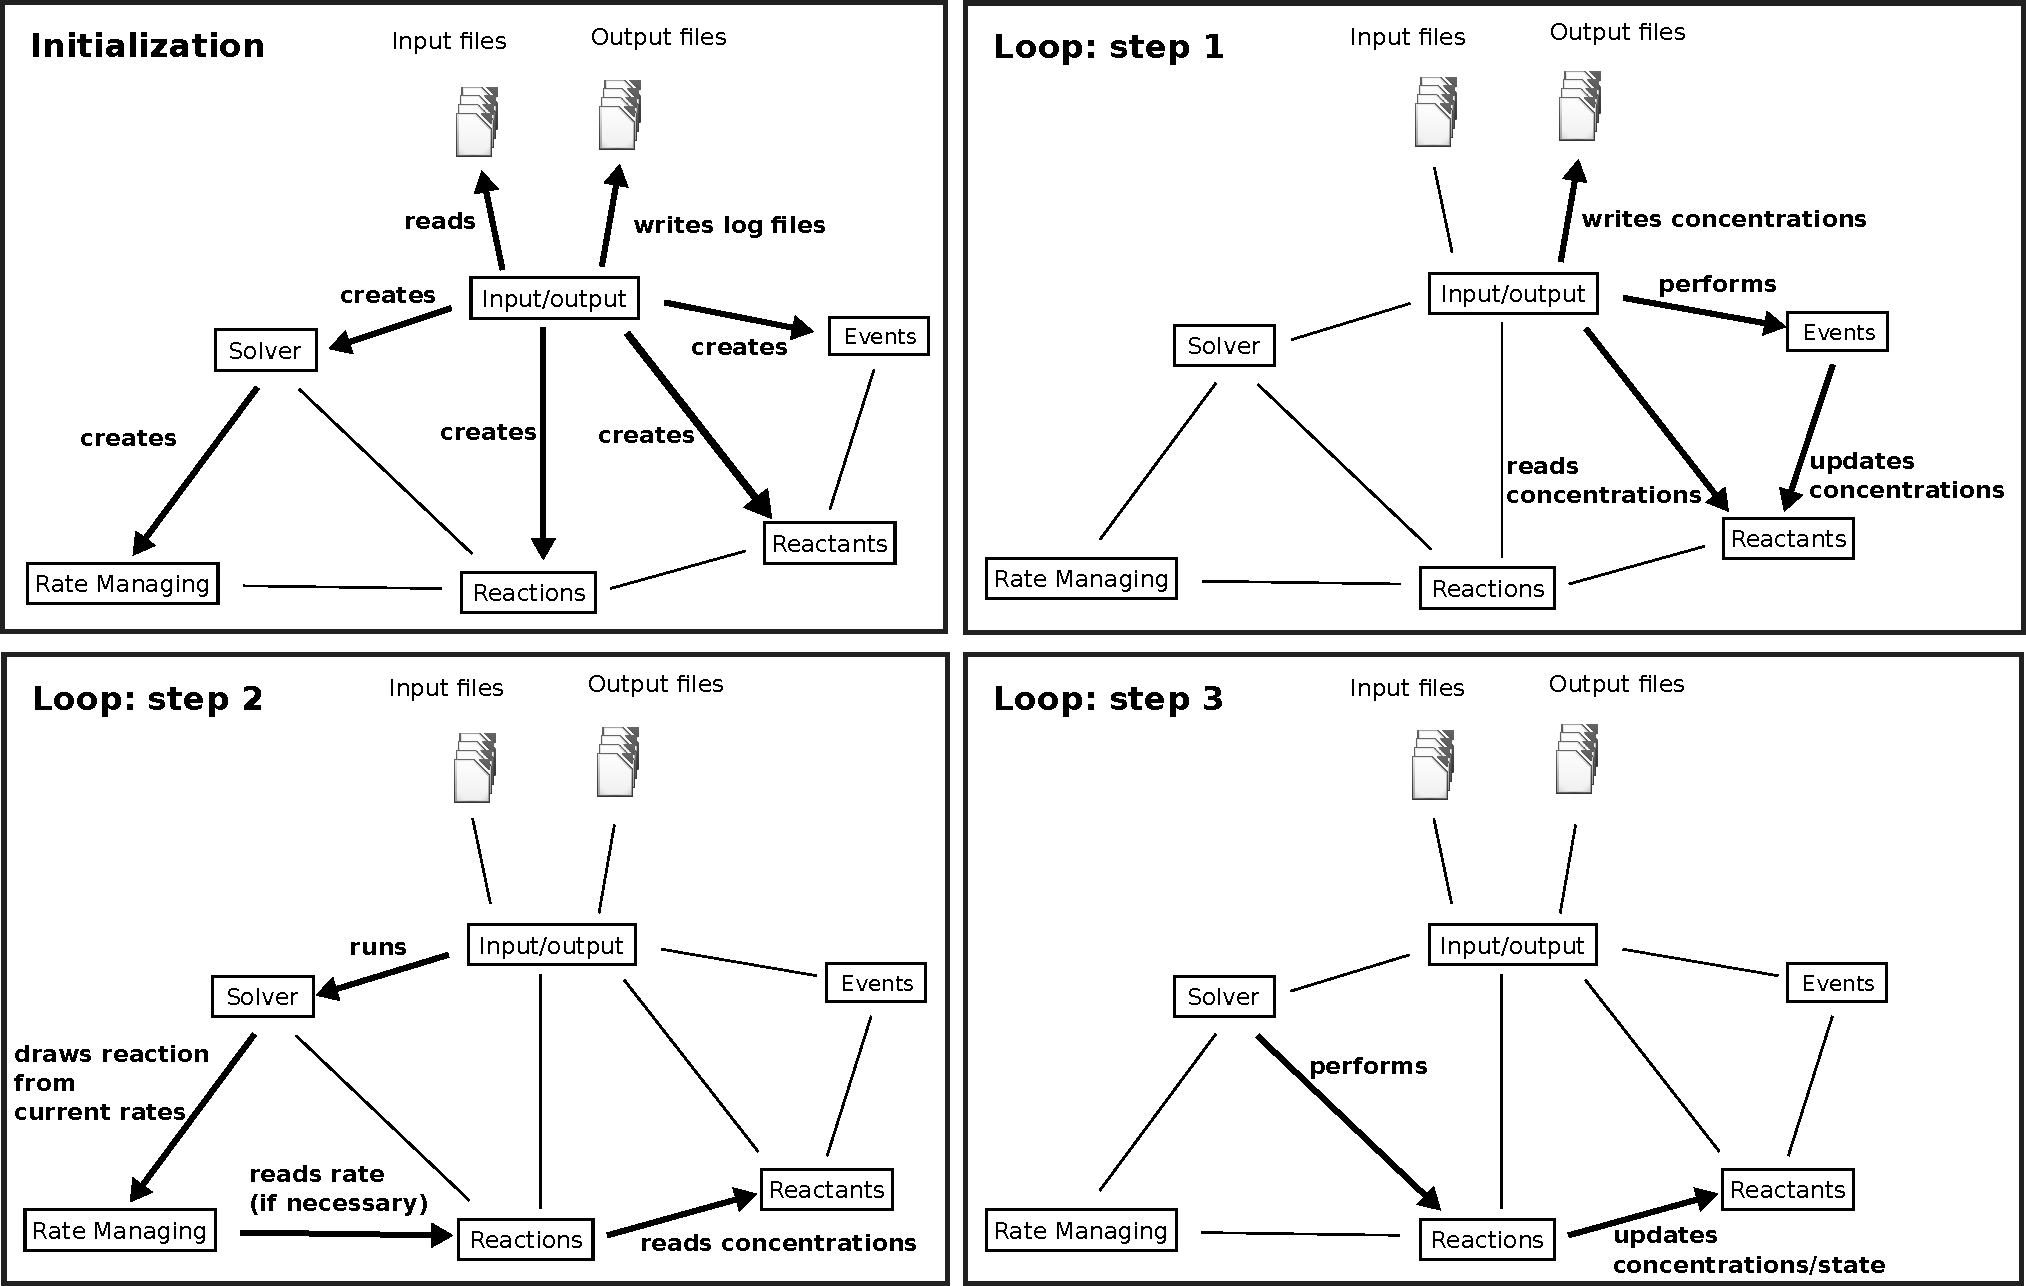
\includegraphics[width=\linewidth]{presentation}
	\caption{Schematical view of the simulator.}
\label{fig:presentation}
\end{figure}

The simulator can be decomposed into several large modules
that handle specific tasks during simulation~\reffigp{fig:presentation}.
First of all, there is an \textbf{input/output} module that creates everything
that is needed for the simulation from an input file.
\textbf{Reactants} and \textbf{reactions} are user-specified and need to be created on demand,
as well as \textbf{events} happening throughout the simulations
and more technical aspects about which algorithm to use to perform the integration.
Once everything is set up, the \textbf{solver} follows a simple loop
that can be decomposed in three steps.
Integration occurs reaction by reaction, at each loop, we go forward one reaction,
update the simulation time, concentrations and reaction rates.

\begin{enumerate}
	\item At the beginning of the loop,
  the \textbf{input/output} process checks whether \textbf{events}
  should occur at the current simulation time and
  whether it needs to write some concentrations to an output file.
	\item It then hands control over to the \textbf{solver},
  which is based on Gillespie's approach to integrate a network of chemical reactions.
  The Gillespie algorithm needs the current reaction rates of all \textbf{reactions}
  and draws a random reaction with a probability proportional to its rate.
  This task is delegated to a \textbf{rate manager},
  which uses state-of-the-art methods to maintain the rate list updated and perform the drawing efficiently.
	\item Once a \textbf{reaction} is drawn, it is performed.
  The concentrations (and the state, see below) of its \textbf{reactants} is modified.
\end{enumerate}


% subsection presenting reactant classes

\subsection{Reactants}

\subsubsection{\texttt{FreeChemical}}

\texttt{FreeChemical} simply represents a pool of interchangeable molecules distributed uniformly in the cell. Computationnally, only the number of molecules in the pool is relevant.

\subsubsection{\texttt{BoundChemical}}

\begin{figure}[!h]
  \centering
  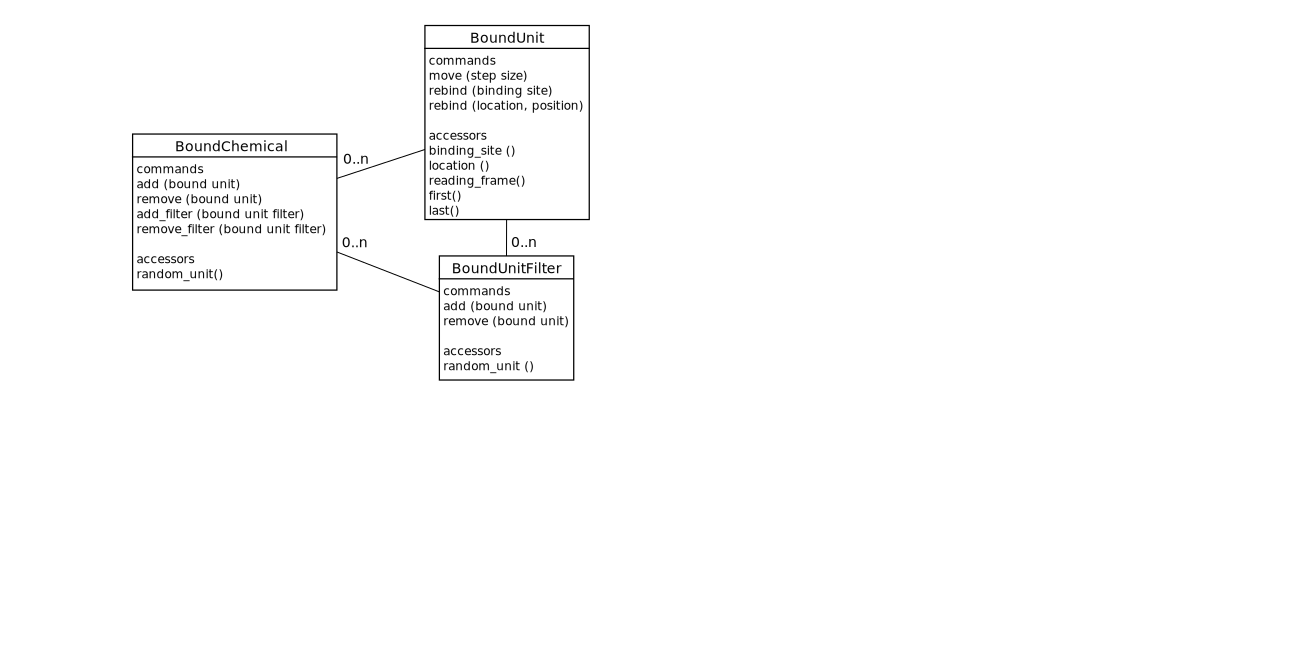
\includegraphics[width=\linewidth]{boundchemical}
  \caption{\texttt{BoundChemical} are in fact a pool of individual \texttt{BoundUnit} created using a \texttt{BoundUnitFactory}. A \texttt{BoundUnit} is characterized by the \texttt{ChemicalSequence} it bound to and its current position. Reaction then use \texttt{BoundUnitFilter} to sort \texttt{BoundUnit} according to some criterium of reference (\textit{e.g.} \texttt{Loading} reactions sort \texttt{BoundUnit} according to the motif they read).}
  \label{fig:bound_chemical}
\end{figure}

\texttt{BoundChemical} represents molecules of the same chemical species, but there are specifities for each unit of a \texttt{BoundChemical}, as all units are bound at different locations of different \texttt{ChemicalSequence}~\reffigp{fig:bound_chemical}. A \texttt{BoundUnitFactory} is used to recycle \texttt{BoundUnit}s, avoiding memory reallocation throughout simulation. \texttt{BoundUnitFilters} are used to sort \texttt{BoundUnit}s according to criteria useful for reactions~\reffigp{fig:bound_chemical}.


\texttt{BoundUnit}s are passed from one \texttt{BoundChemical} species to another through reactions, their attributes are updated if needed. They are only destroyed once they are unbound from their \texttt{ChemicalSequence}.

\subsubsection{\texttt{ChemicalSequence}}

\begin{figure}[!h]
  \centering
  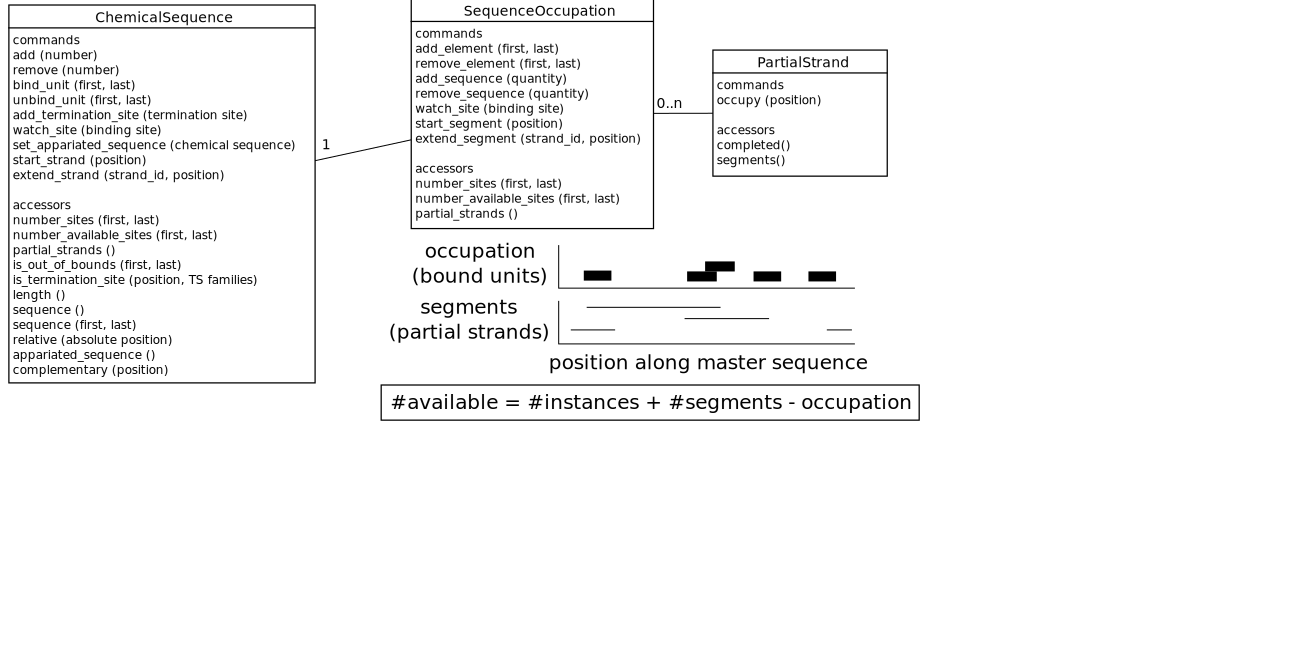
\includegraphics[width=\linewidth]{chemicalsequence}
  \caption{\texttt{ChemicalSequence} represents a pool of polymeres that can be elongated and on which \texttt{BoundUnit}s bind through \texttt{BindingSite}s. For binding to occur, availability of \texttt{BindingSite} is assessed using a utility class \texttt{SequenceOccupation} that records the number of instances of the polymer, the position of \texttt{BoundUnit}s and elongation of \texttt{PartialStrand}s. \texttt{SiteGroup} is used to notify sites of availability changes more efficiently.}
  \label{fig:chemical_sequence}
\end{figure}

\texttt{ChemicalSequence} handles a pool of polymers. A pool is defined by a \emph{master sequence} describing what a typical polymer looks like (\textit{e.g.} the sequence of DnaA protein) and the number of \emph{instances} of the master sequence in the pool. For efficiency reason, we do the following assumptions.

\paragraph{Simplifying assumptions}
\begin{itemize}
\item No deviation from master sequence, all instances are identical.
\item \texttt{BoundUnit}s are not assigned to a specific instance of the sequence, they are positioned on the  master sequence.
\end{itemize}

\subparagraph{Consequences}
\begin{itemize}
\item No direct inference of collisions is possible.
\item A chemical can bind on a partial strand, yet move along the whole sequence freely.
\item Degradation of an instance does not cause unbinding.
\end{itemize}

\paragraph{Site availability}
Despite our simplifying assumptions it is still possible to provide an accurate description of site availability. Availability depends of the number of sequences, number and position of bound elements, number and position of newly polymerized sequence segments~\reffigp{fig:chemical_sequence}.

\subsubsection{\texttt{BindingSiteFamily}}

The task of a \texttt{BindingSiteFamily} is to regroup all the binding sites that can participate in a same \texttt{SequenceBinding} reaction. To simplify the reaction, it stores the subrate associated with each binding site. In order to update the rate properly when availability of sites changes, an \emph{observer pattern} is used~\reffigp{fig:bsf}. 

\begin{figure}[!h]
  \centering
  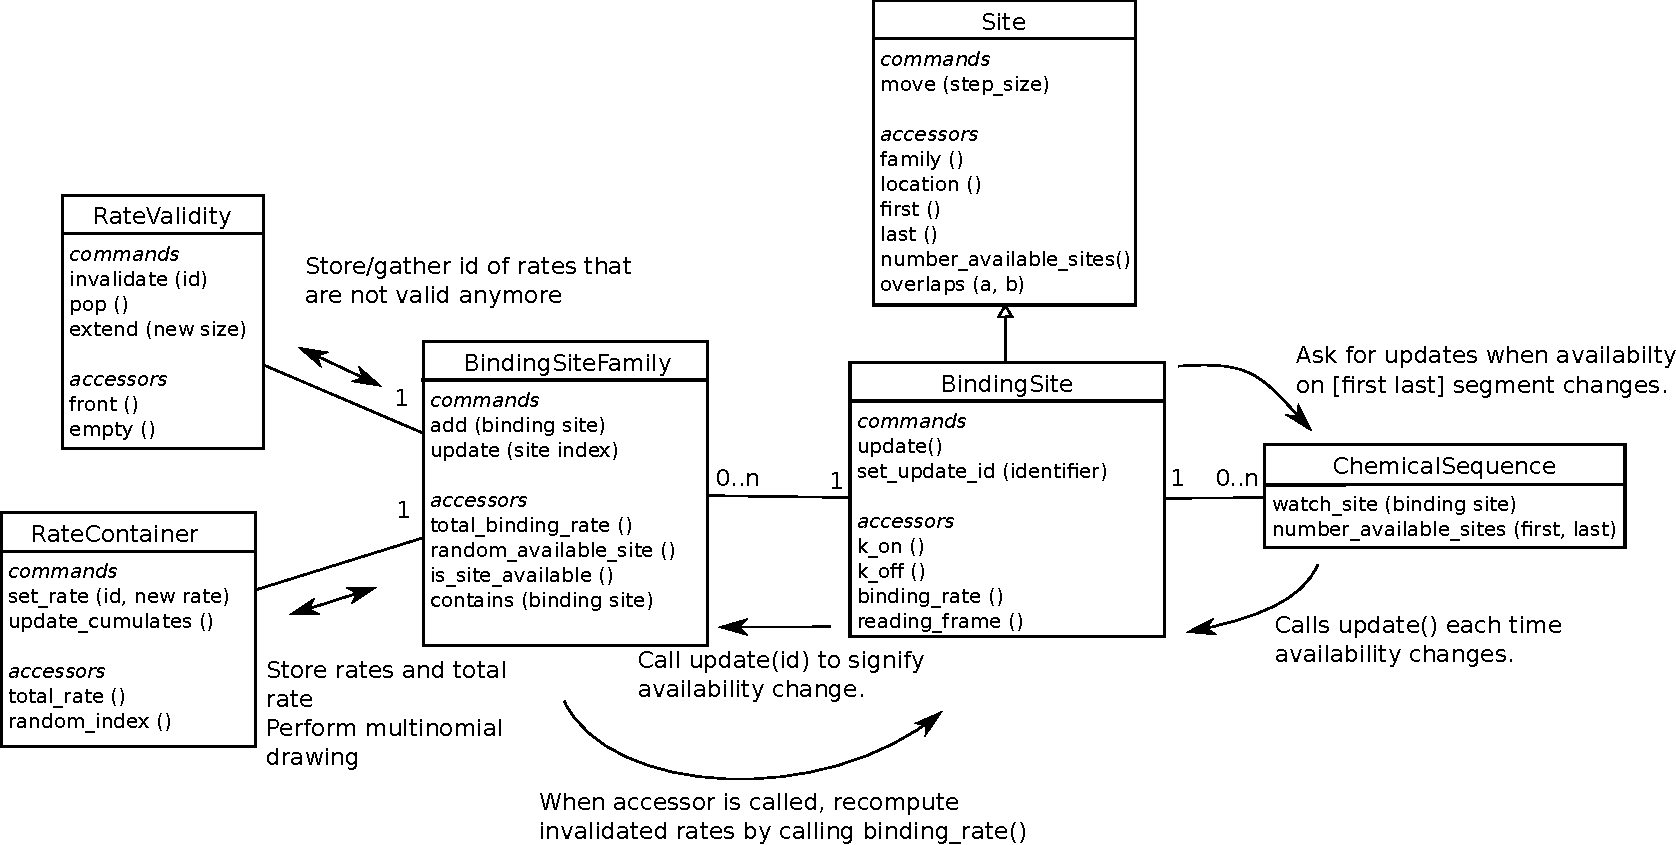
\includegraphics[width=\linewidth]{bindingsitefamily}
  \caption{Schematical view of the Observer pattern used to keep availability of binding sites up to date for \texttt{SequenceBinding} reactions.}
  \label{fig:bsf}
\end{figure}

Every \texttt{BindingSite} is viewed as an \emph{observer} by the \texttt{ChemicalSequence} it belongs to. Every time a change occurs on the site, the \texttt{BindingSite} is notified. The latter binding site notifies its \texttt{BindingSiteFamily} using a specific identifier, letting the family know which binding rate is out of date. This information is stored in a \texttt{RateValidity} class. It is only when it is really needed (\textit{i.e.} when a \texttt{SequenceBinding} wants to access total rate or a random site) that rates are recomputed. This avoids useless computations \textit{e.g.} in the case of a translocation, where a bound unit is first unbound from its \texttt{ChemicalSequence} then rebound. If the bound unit does not move away from the site, two updates will be sent, but the rate will only be recomputed once at the end.

% subsection presenting reaction classes

\subsection{Reactions}

\subsubsection{\texttt{ChemicalReaction}}

Nothing particular.

\subsubsection{\texttt{SequenceBinding}}

\paragraph{Binding} Because of the way \texttt{BindingSiteFamily} is implemented, the reaction can easily and efficiently access the binding rate at all times, no matter what reactions have occured previously and how site availability changed in the meantime.

\paragraph{Unbinding} \texttt{SequenceBinding} uses a \texttt{FamilyFilter} (see detailed description of \texttt{BoundChemical}) to filter out all \texttt{BoundUnit}s that are bound to a binding site of the \texttt{BindingSiteFamily} associated with the reaction. \texttt{BoundUnit}s that have bound to sites of a different family or that have moved away from the binding site through \texttt{Translocation} are \emph{not} candidates for unbiding.

\subsubsection{\texttt{Translocation}}

\paragraph{Collisions} For now, \texttt{Translocation} ignores collisions, making its implementation straightforward.

\paragraph{Stalled form}
\begin{itemize}
  \item Translocation enters stalled form if a \texttt{BoundUnit} reached the end of a sequence.
  \item Translocation enters stalled form if a \texttt{BoundUnit} reaches a termination site \emph{after the translocation was completed}. 
\end{itemize}

\subsubsection{\texttt{Loading}}

\begin{figure}[!h]
  \centering
  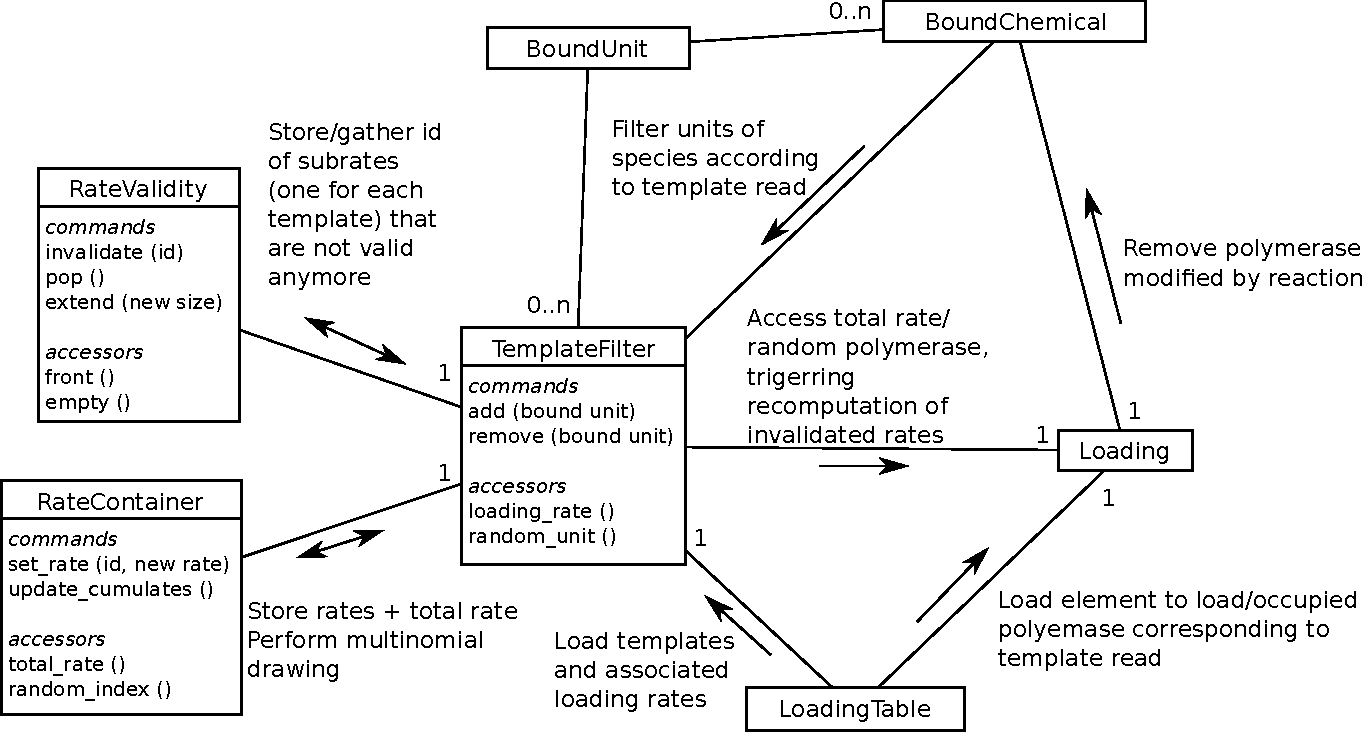
\includegraphics[width=\linewidth]{loading}
  \caption{Schematical view of the pattern used to keep subrates associated with each template up to date in a \texttt{Loading} reaction.}
  \label{fig:det_loading}
\end{figure}

\paragraph{Handling each polymerase individually} The main challenge with \texttt{Loading} is to maintain the subrates associated with each motif up to date. It needs to maintain a list of all \texttt{BoundUnit}s reading a specifing motif. To this end it uses a \texttt{TemplateFilter} (see detailed implementation of \texttt{BoundChemical}). Every time a \texttt{BoundUnit} becomes of the type of the \texttt{BoundChemical} associated with the reaction, the filter looks what motif defined in the \texttt{LoadingTable} it is currently reading. If the motif could not be found, an \texttt{UNKNOWN TEMPLATE} error message is displayed, the \texttt{BoundUnit} is not recorded in the filter and will not participate in the \texttt{Loading} reaction. The implementation is very similar to that used for \texttt{BindingSiteFamily}~\reffigp{fig:det_loading}.

\paragraph{\texttt{ProductLoading} vs \texttt{DoubleStrandLoading}} There difference between the two processes is rather small. We just added a failure condition in the case of \texttt{DoubleStrandLoading} for convenience. Depending on what reactions are used to synthesize a \texttt{DoubleStrand} it might be possible that a polymerase arrives upon a position that has already been synthesized. In this case, the \texttt{DoubleStrandLoading} fails and the polymerase is replaced by the polymerase in its stalled form.

\subsubsection{\texttt{Release}}

\paragraph{Fail polymerase (unknown product)} When a release is triggered, a \texttt{BoundUnit} from the \texttt{BoundChemical} associated with the \texttt{Release} reaction is randomly chosen. Because the \texttt{BoundUnit} knows its current position and its binding site, it will assume that product it has synthesized starts the \emph{reading frame of the binding site} and ends \emph{at the position directly preceding its current reading frame} (we assume that the polymerase translocates onto a terminating sequence which does not contribute to product synthesis). If the product is found in the \texttt{ProductTable}, everything works normally. 

If the product is not found, we display a \texttt{Unknown Product} error message but keep the simulation alive. The fail polymerase in the reaction enables the user to define a rescue pathway. If the release competes with some other reaction for the original polymerase, the fail polymerase can be the original polymerase itself. If products overlap and the polymerase was stalled due to a termination site of another product, fail polymerase can be a polymerase in a sythesizing step (\textit{e.g.} \texttt{ProductLoading}) so synthesis will resume until the next termination site is reached.


\subsection{Switches}

\paragraph{Input format}
\begin{verbatim}
Switch <name> <input_bound_chemical> <output_bound_chemical>
SwitchSite <chemical_sequence> <position> <switch_name>
\end{verbatim}

\texttt{Switch}es are intrinsically linked to \texttt{BoundChemical}s
but apply to specific \texttt{BoundUnit}s through \texttt{SwitchSite}s
located on \texttt{ChemicalSequence}s.
Every time an instance of \texttt{input\_bound\_chemical} steps on a switch site,
it \emph{immediately} becomes an \texttt{output\_bound\_chemical}.

For example, during transcription, an RNA polymerase (RNAP) goes through an
initiation state, then loops through several elongation states
(loading of a nucleotide and translocation).
Once it reaches a termination site represented by a \texttt{SwitchSite},
the RNAP leaves its current elongation state and enters termination state.
It stops performing polymerization reactions and typically releases the polymerization product
and unbinds from DNA.\@

A \texttt{Switch} is not considered a reaction because there is no rate associated with it
(switches are performed automatically before the solver chooses the next reaction).
We dedicate a section to these elements because they play a central role in the simulator's philosophy.
The user can use generic reactions that apply in general
(\textit{e.g.} transcription of any gene based on its sequence)
and use switches every time something more specific is needed.
As seen before, termination sites for transcription are expected to be \textit{SwitchSite}s.
Similarly, important regulation sites can be implemented using \textit{SwitchSite}s.

% subsection presenting solver related classes

\subsubsection{Solver loop}

Once \texttt{Reaction}s and \texttt{Reactant}s are defined, they must be integrated properly. We use variants of the Gillespie algorithm to provide a framework where reactions are performed according to their current reaction rate. Roughly speaking, the main hypothesis of this framework is that reaction timings are distributed according to exponential distributions. This allows for many mathematical simplifications and harmonious integration of an arbitrary number of reactions. The central point of the algorithm is that the probability that a reaction will be the next reaction in the system is proportional to its rate (mathematically speaking, the reaction is obtained by multinomial drawing according to rates).

\begin{figure}[!h]
  \centering
  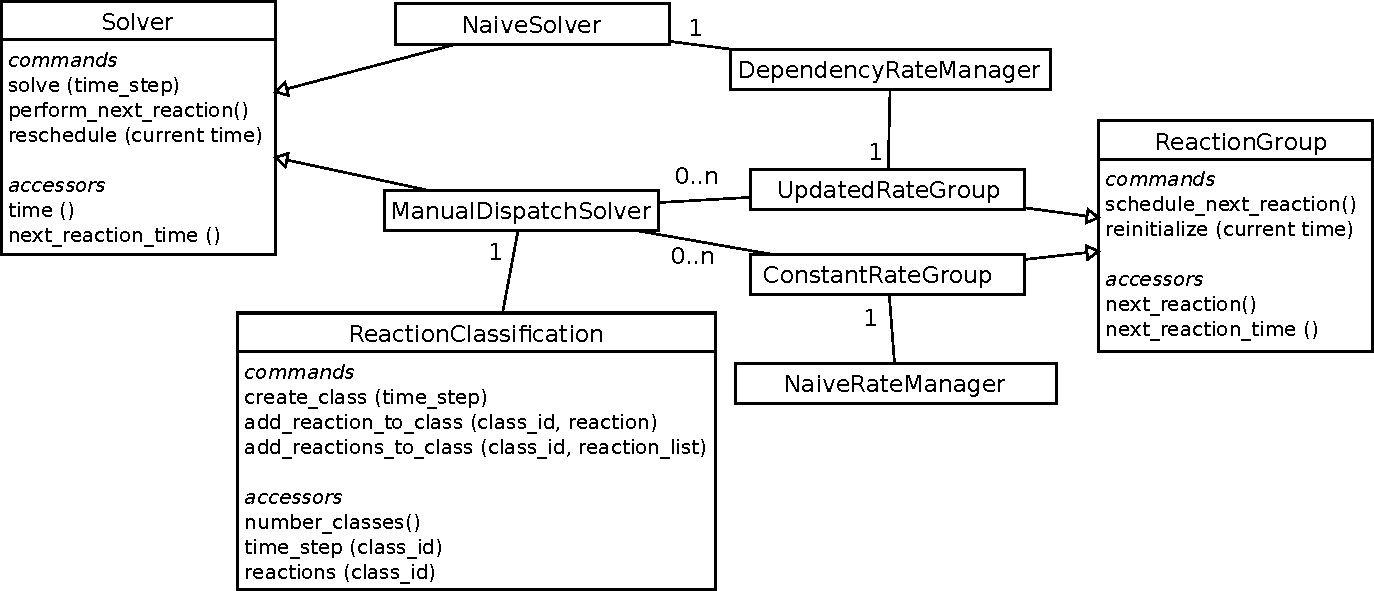
\includegraphics[width=\linewidth]{solver}
  \caption{Solver loop. The loop is driven by the \texttt{Solver} class that defines how and when rates should be updated. The update task is performed by a \texttt{RateManager}. Once rates are known, multinomial drawing is delegated to a \texttt{RateContainer}. A central \texttt{RandomHandler} is used so that the solver only uses one seed, enabling simulation reproducibility.}
  \label{fig:solver}
\end{figure}

The solving loop is depicted in~\reffigt{fig:solver}. The Gillespie algorithm has many variants. We decided to implement it using three \emph{abstract} classes. By using inheritance, variants can be combined for each step of the algorithm (how to update reactions, how to select a reaction). The three central classes are:
\begin{itemize}
  \item \texttt{Solver}: Children of this class decide how and when rates should be updated, \textit{e.g.} update rates after every reaction, only after a given time step, etc. Note that they do not perform any of these computations, they just organize how the algorithm should work.
  \item \texttt{RateManager}: Children of this class are responsible for updating reaction rates when prompted to by a \texttt{Solver} class. Recomputing all rates is generally inefficient, so various implementations of this task can be used to improve the global loop speed.
  \item \texttt{RateContainer}: Childern of this class are responsible for storing reaction rates in a specific structure \emph{adapted} to multinomial drawing. Again many implementations exist, their efficiency depends on the system that is integrated.
\end{itemize}
The implementations of these three classes will be described later in the document.



\subsection{Events}

\texttt{Event}s enable users to change molecule numbers outside of the solver loop at specific times~\reffigp{fig:events}. A \texttt{Simulation} instance handles both a \texttt{Solver} instance and an \texttt{EventHandler} instance. Every time an event timing is reached, the solver loop is stopped, the event(s) is (are) performed, the solver is reinitialized and the simulation resumes. Different \texttt{Event} implementations are offered to modify molecule numbers in a convenient way.

\begin{figure}[!h]
  \centering
  \includegraphics[width=\linewidth]{events}
  \caption{\texttt{Event}s: another way to modify chemical concentrations aside from reactions, \textit{e.g.} to simulate the injection of a chemical inside a cell.}
  \label{fig:events}
\end{figure}

% subsection presenting input/output related classes

\subsection{Input/Output handling}

